\cleardoublepage

\chapter{Servidor de predicción}
\label{makereference5}

\section{Recepción de datos y predicción}

Aunque este servidor sea un componente autónomo del sistema puede estar alojado en la misma máquina que el servidor de datos. Aún así, la comunicación con este se hará a través de un cliente MQTT \ref{makereference3.2} para facilitar la posibilidad de distribuir el sistema en otra topología.

El cliente MQTT estará escuchando continuamente al ``broker'', y en el momento en el que reciba datos, los guardará en un registro diario. Ver figura \ref{log}.

	\begin{figure}[htb]
		\begin{center}
			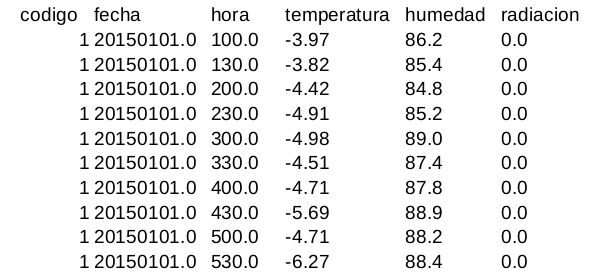
\includegraphics[width=13cm]{figures/log.png}
			\caption{Log del servidor}
		\end{center}
		\label{log}
	\end{figure}

El resultado del entrenamiento del modelo predictivo escogido durante la fase de entrenamiento, ha sido exportado y guardado en este servidor. De esta forma, a la hora de predecir recuperamos este entrenamiento y evitamos volver a realizarlo.

Una vez obtenida la predicción esta es enviada, junto con el resto de datos que recibió el servidor, a nuestro \textbf{sistema de visualización}. 

\section{ThinkSpeak}

Existen distintos sistemas disponibles en el mercado (IoTDataViz, FreeBoard, IBMBlumix...), o incluso podríamos desarrollar uno propio, pero nos hemos decantado por \href{https://thingspeak.com/}{ThinkSpeak}.

\begin{figure}[htb]
	\begin{center}
		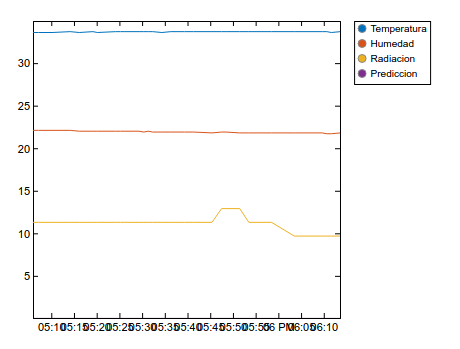
\includegraphics[width=13cm]{figures/ts.png}
		\caption{Gráfica ThingSpeak}
	\end{center}
	\label{ts}
\end{figure}

ThinkSpeak es una plataforma online orientada al ``Internet de las cosas'' (IoT) pensada para almacenar y realizar un seguimiento de los datos obtenidos por distintas aplicaciones.

Una de sus principales ventajas es que los datos recibidos puedes ser procesados por scripts propios implementados en \href{https://es.mathworks.com/products/matlab.html}{MATLAB}. Permitiendo así una observación y manipulación de los datos más personalizada. También cuenta con la ventaja de ser \textbf{gratuita}.

Actualmente, la comunicación con ThinkSpeak se puede realizar nativamente a través de MQTT, sin embargo en el momento de desarrollar la comunicación entre nuestro sistema y este, no contaba con esta característica.

La manera que proporcionaba ThinkSpeak para esta comunicación era a través de \href{https://es.wikipedia.org/wiki/Hypertext_Transfer_Protocol}{HTTP} a través de una \textbf{API REST}. La ventaja que tiene esto, es que cualquier lenguaje que soporte manejo de peticiones HTTP, puede comunicarse con él, permitiéndonos así construir un sistema más modular.

Para realizar el envío de datos a través de esta API, basta con realizar una petición \textbf{HTTP POST} que lleve en el ``body'' (cuerpo de la petición) un campo ``key'' con la clave proporcionada por el servicio y los datos que queremos visualizar.